\scanpage{104}
% archive foliation: 103
\textcircled{1} Carte combinatoire \uline{type}
\figure{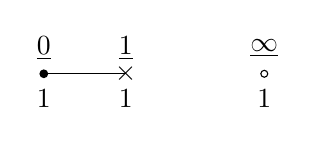
\begin{tikzpicture}[scale=.8]
\draw (0,0)--(1.3,0);\fill (0,0) circle(.07);\node at(1.3,0){$\times$};
\node at(0,.4){$\underline0$};\node at(1.3,.4){$\underline1$};\node at(0,-.4){$1$};\node at(1.3,-.4){$1$};
\draw(3.5,0)circle(.055);\node at(3.5,.4){$\underline\infty$};\node at(3.5,-.4){$1$};
\end{tikzpicture}}
$G\xrightarrow{\sim}\unsure{\gamma}\simeq1\quad\unsure{\delta}=1$
\deleted{$\gamma\simeq\{1\}$}
\margin{$1\quad1\quad1$}
\[f(z)=z\]

\textcircled{2} Carte combinatoire type
\figure{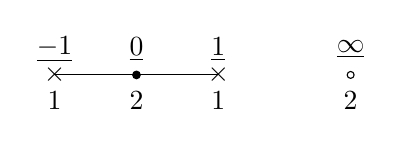
\begin{tikzpicture}[scale=.8]
\draw(-1.3,0)--(1.3,0);\node at(-1.3,0){$\times$};\fill(0,0)circle(.07);\node at(1.3,0){$\times$};
\node at(-1.3,.4){$\underline{-1}$};\node at(0,.4){$\underline0$};\node at(1.3,.4){$\underline1$};
\node at(-1.3,-.4){$1$};\node at(0,-.4){$2$};\node at(1.3,-.4){$1$};\draw(3.4,0)circle(.055);\node at(3.4,.4){$\underline\infty$};\node at(3.4,-.4){$2$};
\end{tikzpicture}}
$G\xrightarrow{\sim}\unsure{\gamma}\simeq\mathbb Z_2\quad\unsure{\delta}=2$
\deleted{$\gamma\simeq\mathbb Z_2$}
\margin{$\begin{array}{ccc}&1&\\2&&2\\&1&\end{array}$}
\[f(z)=z^2\qquad C_{\mathcal C_0}=C^{\alpha}_{\mathcal C_0}\text{ n'a qu'un élément}\ \deleted{\unsure{a}}\]

\textcircled{$2'$} Carte comb. type
\figure{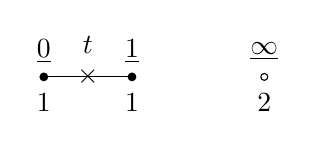
\begin{tikzpicture}[scale=.8]
\draw(0,0)--(1.4,0);\fill(0,0)circle(.07);\node at(.7,0){$\times$};\fill(1.4,0)circle(.07);
\node at(0,.4){$\underline0$};\node at(.7,.5){$\unsure{t}$};\node at(1.4,.4){$\underline1$};\node at(0,-.4){$1$};\node at(1.4,-.4){$1$};\draw(3.5,0)circle(.055);\node at(3.5,.4){$\underline\infty$};\node at(3.5,-.4){$2$};
\end{tikzpicture}}
$G\xrightarrow{\sim}\unsure{\gamma}\simeq\mathbb Z_2\quad\unsure{\delta}=2$
\deleted{$\gamma\simeq\mathbb Z_2$}
\margin{$\begin{array}{ccc}1&&\\&2&2\\1&&\end{array}$}
\[
\left[f(z)=\lambda z(z-1)\qquad
\left\{\begin{array}{l}f(t)=\lambda t(t-1)=1\\f'(t)=\lambda(2t-1)=0\end{array}\right.
\quad\deleted{\unsure{t}}\quad\text{i.e. }t=\tfrac12,\quad\lambda=-4\right]
\]
\[f(z)=-4z(z-1)\]
$C^{\alpha}_{\mathcal C_0}=C_{\mathcal C_0}$ n'a qu'un élément

\textcircled{$2''$}\deleted{\textcircled{$\unsure{2'''}$}}
\deleted{\figure{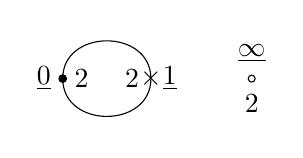
\begin{tikzpicture}[scale=.8]
\draw(0,0) .. controls (0,.8) and(1.4,.8)..(1.4,0) .. controls(1.4,-.8)and(0,-.8)..(0,0);
\fill(0,0)circle(.07);\node at(1.4,0){$\times$};\node at(-.3,0){$\underline0$};\node at(.3,0){$2$};\node at(1.1,0){$2$};\node at(1.7,0){$\underline1$};
\draw(3,0)circle(.055);\node at(3,.4){$\underline\infty$};\node at(3,-.4){$\unsure2$};\end{tikzpicture}}}
$G\xrightarrow{\sim}\unsure{\gamma_2}\xrightarrow{\sim}\mathbb Z_2=\deleted{\unsure{\mathbb Z_2}}\quad\unsure{\delta}=4$
\margin{$\begin{array}{ccc}&&1\\2&2&\deleted4\\&&1\end{array}$}
\deleted{$f(z)=z^2$}
\figure{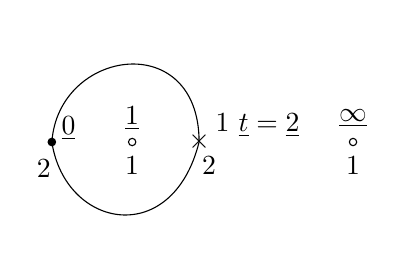
\begin{tikzpicture}[scale=.85]
\draw(0,0)..controls(.1,1.4)and(2.2,1.7)..(2.2,0)..controls(1.8,-1.6)and(.2,-1.3)..(0,0);
\fill(0,0)circle(.065);\node at(2.2,0){$\times$};\node at(.25,.2){$\underline0$};\node at(-.12,-.4){$2$};\node at(2.35,-.35){$2$};\node[right]at(2.3,.25){$\deleted1\ \underline t=\underline2$};
\draw(1.2,0)circle(.055);\node at(1.2,.35){$\underline1$};\node at(1.2,-.35){$1$};\draw(4.5,0)circle(.055);\node at(4.5,.35){$\underline\infty$};\node at(4.5,-.35){$1$};\end{tikzpicture}}
\[
\left[\begin{array}{l}
f(z)=\lambda\dfrac{z^2}{z-1}\\[4pt]
f(t)=\lambda\dfrac{t^2}{t-1}=1\\[4pt]
\left[f'(z)=\lambda\left(\dfrac{2z(z-1)-z^2}{(z-1)^2}\right)=\lambda\dfrac{z^2-2z}{(z-1)^2}=0\right]\\[4pt]
f'(t)=0\qquad t=2\qquad\lambda=\dfrac14
\end{array}\right]
\]
\[f(z)=\frac14\frac{z^2}{z-1}\]
$C^{\alpha}_{\mathcal C_0}$ a un seul él.

\textcircled{$\unsure{3'|3^a}$}
\figure{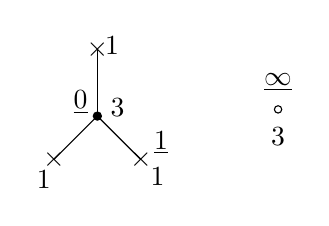
\begin{tikzpicture}[scale=.85]
\draw(0,0)--(0,1);\draw(0,0)--(-.65,-.65);\draw(0,0)--(.65,-.65);\fill(0,0)circle(.07);\node at(0,1){$\times$};\node at(-.65,-.65){$\times$};\node at(.65,-.65){$\times$};
\node at(.22,1.05){$1$};\node at(-.8,-.95){$1$};\node at(.9,-.9){$1$};\node at(.95,-.4){$\underline1$};\node at(-.25,.2){$\underline0$};\node at(.3,.12){$3$};\draw(2.7,.1)circle(.055);\node at(2.7,.5){$\underline\infty$};\node at(2.7,-.3){$3$};\end{tikzpicture}}
$G=\mathbb Z_3\subset\gamma\simeq\mathfrak S_3$
\margin{$\begin{array}{ccc}&1&\\3&1&3\\&1&\end{array}$}
\[f(z)=z^3\]
$C^{\alpha}_{\mathcal C_0}$ a deux éléments, $\gamma$ y est transitif, $\Gamma$ opère via le \unsure{caractère} cyclotomique des \unsure{racines $3$-èmes}.

\textcircled{$\unsure{3''|3^b}$}
\figure{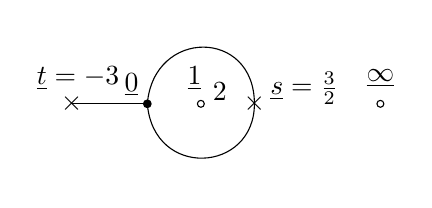
\begin{tikzpicture}[scale=.8]
\draw(-1.2,0)--(0,0);\draw(0,0)..controls(.1,1.2)and(1.7,1.2)..(1.7,0)..controls(1.7,-1.1)and(.1,-1.2)..(0,0);
\fill(0,0)circle(.07);\node at(-1.2,0){$\times$};\node at(1.7,0){$\times$};\node at(-1.1,.4){$\underline t=\unsure{-3}$};\node at(-.25,.3){$\underline0$};\node[right]at(1.8,.25){$\underline s=\frac32$};\draw(.85,0)circle(.055);\node at(.75,.4){$\unsure{\underline1}$};\node at(1.15,.2){$\deleted{\unsure2}$};\draw(3.7,0)circle(.055);\node at(3.7,.4){$\underline\infty$};\end{tikzpicture}}
$G\simeq\mathfrak S_3\qquad\gamma\simeq\{1\}$
\margin{$\begin{array}{ccc}&1&1\\3&2&2\end{array}$}
\[f(z)=\frac4{27}\frac{z^3}{z-1}\qquad\operatorname{Card}C^{\alpha}_{\mathcal C_0}=1\]
